\mychapter{Introdução}\label{ch:introducao}

\section{Apresentação}

% contexto, lacuna, propósito, método, resultados e conclusão:

%Contexto:
A avaliação dos estudantes é uma atividade crucial para o trabalho de um professor, ao permitir avaliar de maneira precisa o desempenho dos estudantes ao longo do curso, fornecendo \textit{feedback} importante para o seu desenvolvimento acadêmico. Além disso, a avaliação também é um meio importante para aprimorar a prática educativa, permitindo que os professores identifiquem pontos fortes e fracos de sua metodologia e aprimorem sua abordagem pedagógica para proporcionar um melhor aprendizado aos estudantes.

% JM - sugestão
%A avaliação é uma prática essencial para todos os professores, pois fornece informações contínuas sobre o desenvolvimento e as dificuldades dos estudantes. Essas informações permitem que os professores identifiquem os pontos fortes e fracos de sua abordagem pedagógica, possibilitando ajustes ou a implementação de novas ações que apoiem o processo de aprendizagem dos estudantes.

% Lacuna:
Avaliar inúmeros estudantes individualizadamente é uma tarefa desafiadora para professores em todos os níveis de ensino, especialmente em disciplinas que exigem habilidades e competências específicas. Esse desafio é ainda maior em exames que envolvem exercícios de programação (EP), uma vez que exigem uma avaliação minuciosa dos processos de resolução de problemas, além da compreensão do código e da lógica utilizados pelos estudantes. Nesse sentido, é fundamental que os professores tenham acesso a ferramentas e técnicas que possam auxiliá-los nessa tarefa, como sistemas de avaliação automatizados e a utilização de exercícios parametrizados. A adoção dessas ferramentas permite uma avaliação mais eficiente das habilidades dos estudantes, garantindo que eles tenham a oportunidade de demonstrar seu conhecimento e habilidades adequadamente.

\subsection{Objetivo} 
Este livro visa disponibilizar uma solução abrangente e eficaz para a avaliação de estudantes. A abordagem colaborativa adotada permite que os professores reutilizem bancos de questões já utilizados por outros colegas que lecionam na mesma disciplina, economizando tempo e esforço na criação de avaliações personalizadas.

Essa metodologia pode ser aplicada tanto em exames unificados em várias turmas com milhares de estudantes, quanto em disciplinas com turmas menores ministradas por um único professor.

\subsection{Método} 
Para ajudar professores a avaliar os estudantes, este livro apresenta o MCTest, um sistema de código aberto que permite a elaboração e correção de exames com questões de múltipla escolha (QMs) ou dissertativas (QTs), incluindo EP. Esse sistema oferece questões parametrizadas e exames individualizados, que podem ser utilizados por várias turmas simultaneamente. O MCTest foi inicialmente desenvolvido para corrigir exames em processos seletivos para um curso de especialização na Universidade Federal do ABC (UFABC) em 2012, mas evoluiu significativamente para uma versão inteiramente web.

O MCTest pode ser integrado a Ambientes Virtuais de Aprendizagem (AVAs), como o Moodle, o qual é uma plataforma digital que oferece uma variedade de recursos e ferramentas para melhorar o processo de ensino e aprendizagem. Os AVAs podem ser usados como um complemento ou suporte às aulas presenciais, ou como uma opção para o ensino a distância (EaD). Eles oferecem um espaço virtual no qual estudantes e professores podem interagir, acessar materiais didáticos, realizar atividades, participar de fóruns de discussão e avaliações. Esses ambientes proporcionam aos estudantes maior flexibilidade para acessar o conteúdo e realizar suas tarefas em horários mais convenientes, o que também permite uma maior personalização do processo de aprendizagem.

Assim, este livro ensina como criar exames individualizados, com questões parametrizadas, intercalando textos em \LaTeX{} e códigos em Python, e correção automática. Essas questões podem incluir EPs utilizando o \textit{plugin} VPL (\href{https://vpl.dis.ulpgc.es/}{\textit{Virtual Programming Lab}}) no Moodle.
No entanto, antes de elaborar esses EPs, é importante discutir como navegar pelo sistema utilizando um dos seus três tipos de usuários: administrador, coordenador de disciplina e professor. Mesmo um professor sem habilidade de programação pode utilizar o MCTest para criar exames com questões estáticas, em que a única variação é o sorteio das questões e das alternativas. Cada tipo de usuário possui um conjunto de funcionalidades para criar e alterar as diversas entidades do sistema, incluindo Instituto, Curso, Disciplina, Tópico, Questão, Turma, Professor, Estudante e Exame.

O MCTest já foi implantado com sucesso na UFABC e serve como plataforma para os professores e gestores da instituição. O leitor pode examinar a implantação deste sistema em \href{http://mctest.ufabc.edu.br}{mctest.ufabc.edu.br} para entender melhor como o sistema funciona e como pode ser utilizado para aprimorar a avaliação de habilidades dos estudantes.

\subsection{Resultados} 
O livro apresenta os resultados de dezenas de experimentos realizados ao longo dos últimos 12 anos em disciplinas na UFABC. Os experimentos foram realizados em disciplinas como Bases Computacionais da Ciência, Processamento da Informação, Programação Estruturada, Processamento Digital de Imagens e Visão Computacional, tanto nos Bacharelados em Ciência e Tecnologia (BCT) e Ciência da Computação (BCC), quanto na pós-graduação em Ciência da Computação. Além disso, o livro também relata um experimento realizado na disciplina de Funções de Uma Variável (Cálculo) no BCT, utilizando a biblioteca \href{http://sympy.org}{sympy.org} para questões algébricas.

Este livro apresenta os resultados de experimentos conduzidos em três modalidades: híbrida, totalmente remota e totalmente presencial. Foram selecionados os melhores resultados obtidos por meio de artigos e registros de software, os quais estão disponíveis para consulta em \href{http://vision.ufabc.edu.br}{vision.ufabc.edu.br}. Os experimentos demonstram a eficácia do método avaliativo utilizando o MCTest na avaliação de disciplinas de computação, bem como em processos seletivos gerais.

% Conclusão:
Com o sistema MCTest apresentado neste livro, os professores têm à disposição uma ferramenta poderosa para aprimorar a avaliação de habilidades e competências dos estudantes em programação. Ao utilizar o MCTest, os professores podem minimizar o esforço de criar e corrigir exames e EPs, permitindo que se dediquem a atividades de ensino menos repetitivas e mais significativas.

Além disso, o MCTest oferece uma avaliação mais eficiente, tornando o processo de avaliação menos suscetível a erros humanos e mais preciso. Isso pode proporcionar uma experiência de aprendizado mais satisfatória para os estudantes, que se sentirão mais seguros e motivados a progredir em suas habilidades.
 
% \noindent
% \textbf{Palavras-chave:} Avaliação automatizada, Avaliação parametrizada, Ensino de Programação, MOOC.

% \begin{mybox}{corObs}{\textbf{Observação:\\\vspace{-3mm}\hrule\vspace{3mm}}}
% Os textos apresentados neste livro foram adaptados de conversas com modelos de inteligência artificial (IA) disponíveis em \href{https://poe.com/}{poe.com}. 
% \\\\
% Por exemplo, os próximos três parágrafos em itálico constituem uma resposta gerada pela IA em resposta a uma solicitação específica para expandir o parágrafo anterior. Essa solicitação foi feita após várias consultas em diferentes partes dos Capítulos \ref{ch:introducao} -- \nameref{ch:introducao} e \ref{ch:visaoGeral} -- \nameref{ch:visaoGeral} deste livro. É importante ressaltar que a resposta fornecida por \textit{chatbot} não pode ser considerada uma conversa real, pois apenas responde a uma solicitação e não faz perguntas adicionais para aprofundar a compreensão do contexto. Portanto, trata-se de uma resposta específica a uma solicitação, e não de uma conversa propriamente dita.

% \end{mybox}

% \begin{mybox}{corCopia}{\textbf{Resposta de \href{https://poe.com/ChatGPT}{poe.com/ChatGPT}:\\\vspace{-3mm}\hrule\vspace{3mm}}}

% {\em\color{black}
% Poe.com é um site que oferece acesso a vários modelos de inteligência artificial para conversação, incluindo chatbots e modelos de linguagem, por meio de uma interface amigável ao usuário. Os usuários podem inserir textos de entrada e receber respostas geradas pelos modelos de IA, treinados em grandes conjuntos de dados de linguagem humana.
% \\\\
% Os textos apresentados neste livro foram adaptados de conversas com esses modelos de IA, usando as respostas geradas pelos modelos como ponto de partida para uma edição e refinamento adicionais por autores humanos. O objetivo foi criar conteúdo informativo e envolvente que aproveite as capacidades dos modelos de IA, ao mesmo tempo, em que incorpora a criatividade e a expertise dos autores humanos.
% \\\\
% Ao utilizar modelos de IA dessa maneira, esperamos demonstrar o potencial dessas tecnologias para aprimorar o processo de criação de conteúdo e fornecer novas oportunidades de colaboração entre autores humanos e máquinas inteligentes.}
% \end{mybox}

\section{Breve histórico do MCTest}\label{sec:historico}

Nesta seção, será apresentado um breve histórico do MCTest. Essa ferramenta surgiu como resposta à necessidade do curso de Especialização em Tecnologias e Sistemas de Informação (TSI) Lato Sensu da UFABC. Este curso foi pioneiramente oferecido pela universidade em 2010 (TSI-1). Desde a sua segunda edição (TSI-2), em 2012, o MCTest tem sido amplamente utilizado em diversos processos seletivos e exames de disciplinas, desempenhando um papel fundamental também na Escola Preparatória da UFABC (EPUFABC).

Ao longo deste livro, os experimentos realizados com o MCTest serão descritos em detalhes, abrangendo diversos aspectos de seu uso e aplicação. Caso haja interesse em conhecer mais sobre o uso do MCTest em processos seletivos, exames de disciplinas ou na Escola Preparatória da UFABC, basta consultar os capítulos específicos dedicados a esses temas.

\subsection{MCTest no TSI}

O curso TSI-1 estabeleceu uma parceria com o programa Universidade Aberta do Brasil, vinculado ao Ministério da Educação (UAB/MEC), e oferecido na modalidade de ensino a distância (EaD), com exames presenciais correspondendo a mais de 50\% da nota de aprovação do estudante. Em 2010, houve 1078 candidatos para as 200 vagas disponíveis em quatro polos do estado de São Paulo, com 16 tutores no total. 

A segunda edição do curso (TSI-2) iniciou em 2012, com 1171 inscritos distribuídos em 4 polos, contendo 50 estudantes em cada polo. No entanto, apenas 674 candidatos concluíram o processo seletivo \cite{2013:Zampirolli.Quilici-Gonzalez.ea}. Nesta edição, foi desenvolvida a primeira versão do MCTest, como será detalhada na próxima seção.


Na terceira oferta, em 2014 (TSI-3), foram 689 candidatos para 6 polos, com 300 estudantes matriculados. No início, houve 11 tutores, porém, na fase do TCC, em 2015, o número total de tutores aumentou para 16. 

A quarta edição do curso (TSI-4) ocorreu em 2017, porém sem as bolsas UAB para professores e tutores. Como resultado, foram oferecidas apenas duas turmas, nos polos da UFABC em Santo André (SA) e São Bernardo do Campo (SBC), com 25 estudantes em cada polo e sem a presença de tutores. Apesar disso, a demanda permaneceu alta, com 863 inscritos para apenas 50 vagas disponíveis nessa edição.

Até a quarta edição do TSI, a parte administrativa do curso era conduzida pela Pró-Reitoria de Extensão. Durante a fase de transição dos cursos de especialização para a Pró-Reitoria de Pós-Graduação, houve um intervalo maior entre as edições do curso, que foi agravado pela pandemia de COVID-19. Como resultado, somente no segundo semestre de 2022 foi possível iniciar o TSI-5, também sem as bolsas UAB, com apenas 25 estudantes em cada polo da UFABC em SA e SBC. Nessa edição, talvez devido à pandemia, apenas 63 candidatos participaram do processo seletivo, em contraste com a edição anterior, que teve uma média de 17,26 candidatos por vaga.

No início de 2023, deu-se início à sexta edição do TSI (TSI-6), que agora conta com o retorno das bolsas UAB. Essa edição está sendo conduzida em paralelo com a TSI-5 e conta com a colaboração de 7 tutores. Ao todo, foram registrados 565 candidatos para os 6 polos do estado de São Paulo, resultando em uma média de 35 estudantes por polo.

\subsection{Versões do MCTest}\label{sec:registrosSoftware}

O MCTest é um projeto que evoluiu ao longo do tempo, e isso pode ser visto nas diferentes versões registradas no Instituto Nacional de Propriedade Intelectual (INPI). Cada versão registra uma evolução do projeto em termos de tecnologia, metodologia e objetivos.

A primeira versão do MCTest (MCTest-1) foi registrada no INPI com o número de registro BR 51 2013 001231 7. Essa versão foi desenvolvida em Matlab para permitir a correção automática dos exames gerados em Word ou BROffice. O MCTest-1 foi utilizado nos processos seletivos do TSI de 2012 até 2017, contribuindo significativamente para a avaliação das competências cognitivas dos candidatos.

Foi desenvolvida uma versão do MCTest denominada MCTest-2 em colaboração com um estudante de Iniciação Científica, e essa versão foi devidamente registrada no INPI sob o número de registro BR 51 2015 001444 7. Essa versão específica, disponibilizada para dispositivos Android, possibilitou a correção automática dos exames gerados em Word ou BROffice \cite{2014:China.Zampirolli,2015:Zampirolli.China.ea,2016:China.Zampirolli.ea}.

A versão MCTest-3 foi desenvolvida em Python e registrada no INPI com o número de registro BR 51 2015 001445 5. Assim como as versões anteriores, essa versão também permitia a correção automática de exames gerados em Word/BROffice.

Já a versão MCTest-4, registrada no INPI com o número de registro BR 51 2016 001344 3, foi desenvolvida em Python e também permitia a correção automática dos exames. No entanto, os exames foram digitalizados e enviados por FTP para o servidor \href{http://vision.ufabc.edu.br}{vision.ufabc.edu.br}, com os exames gerados pela versão MCTest-4.G \cite{2016:Zampirolli.Batista.ea}. Essa versão representou um avanço significativo em relação às anteriores, ao permitir o envio remoto dos exames digitalizados e a correção automática, simplificando o processo de avaliação dos candidatos. Essa versão está disponibilizada em \href{https://github.com/fzampirolli/mctest4}{github.com/fzampirolli/mctest4} \cite{2016:Zampirolli.Batista.ea}.

Posteriormente, entre maio e agosto de 2018, foi desenvolvida e lançada a versão atual do MCTest, a MCTest-5.2. Essa versão apresentou grandes mudanças, sendo disponibilizada em páginas web e desenvolvida em Python com IDE Django, permitindo a geração e correção automática de exames. A MCTest-5.2 está disponível em  \href{https://github.com/fzampirolli/mctest}{github.com/fzampirolli/mctest}, com os exames gerados em \LaTeX \ e usando o banco de dados MySQL. Desde o seu lançamento, essa nova versão gerou diversas publicações, a partir de 2018, que podem ser acessadas através do site \href{http://vision.ufabc.edu.br}{vision.ufabc.edu.br}. 

A grande contribuição do MCTest ao estado da arte em exames avaliativos e formativos está na possibilidade de criar questões parametrizadas, intercalando descrições em \LaTeX \ com códigos em Python, disponível a partir da versão MCTest-4.G. Os exames gerados com essas questões podem ter a correção automática com: 

\begin{enumerate}
    \item Exames digitalizados e enviados para o MCTest; 
    \item Se forem questões de exercícios de programação (EPs), com respostas dadas em código em alguma linguagem de programação, o MCTest gera um arquivo com os casos de teste e outro com a variação de cada estudante. Esses arquivos devem ser inseridos em atividades VPL no Moodle para a correção automática; 
    \item Outra possibilidade é o MCTest exportar um banco de questões em formato Aiken ou XML, que podem ser importados pelo Moodle para criar exames. 
\end{enumerate}

O Moodle também aceita questões paramétricas, mas são limitadas ao conjunto de funções do PHP, como relatado no artigo de \citeonline{2021:Zampirolli.Batista.ea*1}.

\subsection{MCTest nos processos seletivos e exames de disciplinas do TSI}

Desde 2012, todos os processos seletivos do TSI têm sido realizados com o uso do MCTest. Até a versão MCTest-4, os exames eram criados em editores de texto, como Word ou BROffice. A partir da versão MCTest-4G, no entanto, os exames começaram a ser criados diretamente pelo sistema.

Além disso, os professores da disciplina de Processamento de Informação (CS1) do Bacharelado em Ciência e Tecnologia da UFABC, na modalidade semipresencial, viram a oportunidade de utilizar o sistema em questões contendo EP, como relatado no artigo de \citeonline{2018:Zampirolli.Goya.ea}. Com o passar do tempo, várias outras turmas e professores também começaram a utilizar o sistema e a sugerir melhorias.

Desde 2012, todas as 13 disciplinas do TSI tiveram seus exames presenciais corrigidos com o auxílio do MCTest. A partir de 2017, os exames também passaram a ser gerados pelo sistema, sendo reaproveitados em cada nova oferta, com pequenas modificações. Essa mudança representou uma significativa melhoria na eficiência e rapidez do processo de avaliação, além de permitir a personalização e adaptação dos exames para cada nova oferta.

\subsection{MCTest na Escola Preparatória}

A UFABC oferece gratuitamente à comunidade da região do ABC um curso preparatório para vestibulares chamado Escola Preparatória da UFABC (EPUFABC). Desde 2017, o MCTest tem sido um importante aliado no processo seletivo dos candidatos da EPUFABC. Esses processos atraem milhares de candidatos para as cerca de 300 vagas disponíveis anualmente.

Para viabilizar esse processo, foi empregado o MCTest para gerar o quadro de respostas (QR) dos candidatos, enquanto as QMs foram impressas separadamente. O uso do MCTest mostrou-se fundamental para agilizar e simplificar o processo seletivo, permitindo a correção automática dos exames e a rápida geração do resultado. Além disso, a precisão e confiabilidade do sistema garantiram uma avaliação sem erros dos candidatos, contribuindo para a excelência acadêmica da UFABC e o sucesso dos estudantes matriculados na EPUFABC.

Essa parceria permitiu o desenvolvimento de mais um sistema (ENEM Interativo) e a publicação de dois artigos, os quais serão resumidos a seguir e detalhados na Parte \ref{part:experimentos} de experimentos.

\subsubsection{ENEM Interativo}\label{sec:enemInterativo}

Em colaboração com a EPUFABC, foi desenvolvido um sistema interativo denominado \href{http://mctest.ufabc.edu.br:8000/ENEM}{ENEM interativo}, permitindo que os estudantes utilizem exames antigos do ENEM e os microdados disponibilizados pelo INEP para estudo. Nesse sistema, os exames em formato PDF são convertidos para HTML, e botões de resposta são incluídos para cada questão. Ao término de cada exame, o botão de estatísticas abre uma nova página contendo dados do gabarito, respostas dos estudantes, habilidades (valores fornecidos pelo INEP) e gráficos.

Esses gráficos mostram a Curva Característica do Item (CCI) da Teoria de Resposta ao Item (TRI) \cite{birnbaum1968some}, sendo calculada a partir dos parâmetros da amostra aleatória de 10.000 estudantes, incluindo a discriminação (a), habilidade (b) e chute (c). Os valores médios e o desvio padrão da amostra também são calculados, permitindo uma melhor compreensão da distribuição dos resultados.

Outro gráfico gerado é o BoxPlot \cite{jw1977exploratory}, juntamente com o ViolinPlot \cite{hintze1998violin}, para visualizar as frequências de acertos (valor 1) e erros (valor 0) de forma mais clara e precisa.

É importante ressaltar que esses gráficos estão disponíveis apenas para exames com respostas de mais de 10.000 estudantes. Essa ferramenta tem sido uma contribuição para o processo de preparação dos estudantes para o ENEM, fornecendo informações valiosas sobre o desempenho dos estudantes e as tendências de cada questão ao longo do tempo \cite{2021:Zampirolli.Junior.ea}.

\subsubsection{Comparações de três métodos de seleção}

Foi realizado um estudo comparativo entre três métodos de seleção de candidatos para a EPUFABC: 1) o uso do MCTest com exames presenciais, aplicando a Teoria Clássica ao Item (TCI); 2) o uso do Moodle durante a pandemia de COVID-19, com a realização dos exames a distância, também utilizando a TCI; e 3) o uso do MCTest com exames presenciais, empregando a TRI. 

Os resultados obtidos indicaram que, ao adotar a TRI, as chances de empate entre candidatos foram consideravelmente reduzidas. Adicionalmente, foi constatado que a correlação entre as classificações obtidas pelos métodos TCI e TRI é alta, evidenciando coerência entre os dois métodos de pontuação \cite{2021:Zampirolli.Batista.ea}.


\section{Direitos autorais}

Nesta seção, serão abordados os direitos autorais do software e das questões criadas pelos professores e disponibilizadas no banco de dados do MCTest.

\subsection{Direitos autorais do software}

Até a primeira edição deste livro, o MCTest foi desenvolvido integralmente pelo Prof. Francisco de Assis Zampirolli, da Universidade Federal do ABC (UFABC), visando atender às demandas da instituição na avaliação de inúmeros estudantes e candidatos de processos seletivos. O sistema contou com a valiosa colaboração de colegas da UFABC, que compartilharam suas necessidades em relação às avaliações. No entanto, é crucial ressaltar que o MCTest não é um produto comercial e, infelizmente, não segue rigorosamente o ciclo de vida de desenvolvimento de software.

Trata-se de um sistema construído inspirado no modelo de prototipagem de Engenharia de Software. Para vir a se tornar um produto comercial, seria necessário submetê-lo a uma engenharia reversa e aprimorá-lo, sobretudo no que concerne à navegabilidade entre as telas e à adição de mais funcionalidades de gestão de processos. 

Mesmo com as limitações mencionadas anteriormente, o MCTest está em produção na UFABC e é utilizado por professores e gestores para avaliar milhares de estudantes e candidatos, reduzindo significativamente a parte repetitiva dos processos de avaliação.

O MCTest possui código aberto e está disponível no \href{https://github.com/fzampirolli/mctest}{GitHub}, podendo ser usado e modificado sob a licença AGNU. Isso implica que todos têm a liberdade de utilizar o sistema. Para manter o MCTest atualizado, melhorias feitas por terceiros e implementadas em seus servidores também devem ser compartilhadas com o público. Essa licença pode ser encontrada na implantação na UFABC em \href{http://mctest.ufabc.edu.br/license}{mctest.ufabc.edu.br/license} e também está apresentada a seguir:

\begin{mybox}{corCopia}{\textbf{Licença:\\\vspace{-3mm}\hrule\vspace{3mm}}}
{\em Copyright (C) 2018-2023 Francisco de Assis Zampirolli from Federal University of ABC and individual contributors. All rights reserved.
This file is part of MCTest 5.2.
Languages: Python, Django, and many libraries described at
\href{https://github.com/fzampirolli/mctest}{github.com/fzampirolli/mctest}.
\\\\
You should cite some references included in \href{http://vision.ufabc.edu.br}{vision.ufabc.edu.br} in any publication about it.
\\\\
MCTest is free software: you can redistribute it and/or modify it under the terms of the GNU Affero General Public License (\href{http://gnu.org/licenses/agpl-3.0.txt}{gnu.org/licenses/agpl-3.0.txt}) as published by the Free Software Foundation, either version 3 of the License or (at your option) any later version.
\\\\
MCTest is distributed in the hope that it will be useful, but WITHOUT ANY WARRANTY; without even the implied warranty of MERCHANTABILITY or FITNESS FOR A PARTICULAR PURPOSE. See the GNU General Public License for more details.}
\end{mybox}

\subsection{Direitos autorais das questões disponíveis no BD}\label{sec:deAcordo}

Outro ponto muito importante a respeito dos direitos autorais refere-se às questões elaboradas no MCTest e armazenadas em seu banco de dados (BD). A filosofia do MCTest é trabalhar colaborativamente para produzir e utilizar material didático em avaliações. Dessa forma, as questões elaboradas por um professor em uma disciplina da UFABC estão disponíveis para os demais professores desta disciplina, para uso exclusivo em suas avaliações nesta universidade. 

Cada instituição pode definir seus próprios critérios de direito autoral para o conteúdo disponibilizado no BD do MCTest. É importante ressaltar que o direito autoral do software apresentado na seção anterior não cobre essa parte. Portanto, cabe a cada instituição definir seus próprios critérios em suas implantações do MCTest.

A seguir, será apresentado o que foi definido para os professores da UFABC que optaram por utilizar o sistema na implantação disponibilizada em \href{http://mctest.ufabc.edu.br/According}{mctest.ufabc.edu.br/According}.

\begin{mybox}{corCopia}{\textbf{De Acordo:\\\vspace{-3mm}\hrule\vspace{3mm}}}
O MCTest (disponível gratuitamente no \href{https://github.com/fzampirolli/mctest}{GitHub}) foi implantado no servidor da UFABC: \href{http://mctest.ufabc.edu.br}{mctest.ufabc.edu.br}.
\\\\
Na UFABC, o MCTest é um serviço colaborativo para geração e correção automática de atividades de formação (como Listas de Exercícios) e de avaliação (como Testes ou Exames).
\\\\
Esse serviço está disponível gratuitamente para todos os docentes da UFABC.
\\\\
Para poder utilizar o MCTest, o professor deve inscrever-se na plataforma e ser cadastrado em alguma disciplina pelo seu coordenador.
\\\\
Todo o material intelectual (aulas, vídeos, questões, etc.) disponível neste site está protegido pelo direito autoral dos seus respectivos autores e, em última instância, é propriedade da UFABC. Os autores proprietários do material disponibilizado no site concordam em liberar o seu uso sem restrições pelos professores da instituição a qual está vinculado somente no âmbito das disciplinas e cursos desta instituição. Além disso, quando me inscrevo neste serviço, nesta instituição, CONCORDO que:
\begin{itemize}
    \item Posso utilizar livremente em meus exames todas as questões disponíveis já cadastradas na disciplina;
    \item Não posso publicar questões criadas por outros professores em quaisquer outras mídias, como, por exemplo, livros e artigos;
    \item Todas as novas questões que eu criar podem ser reaproveitadas em exames elaborados por outros professores da mesma disciplina, sem prévio aviso;
    \item Só posso mudar as questões dos outros professores SOMENTE SE HOUVER ALGUM ERRO. Porém, sem alterar a autoria da questão.
\end{itemize}

\end{mybox}

\section{Instalando o MCTest}\label{sec:instalacao}

O MCTest pode ser instalado localmente no computador pessoal utilizando a máquina virtual \href{https://www.virtualbox.org/}{VirtualBox}. Em seguida, é necessário baixar uma das seguintes versões do Linux: Ubuntu 20.04 ou 22.04, ou ainda a distribuição Mint 21 Mate. Essas distribuições já foram testadas, mas o MCTest pode funcionar em outras também.

Após instalar o Linux na máquina virtual ou utilizá-lo diretamente em uma instalação Linux, sem a máquina virtual, basta fazer o \textit{download} do arquivo \href{https://raw.githubusercontent.com/fzampirolli/mctest/master/_setup-all.sh}{\texttt{\_setup-all.sh}}, disponível no endereço \href{https://github.com/fzampirolli/mctest}{github.com/fzampirolli/mctest} do GitHub, e executá-lo em um terminal com privilégios de superusuário (\verb|sudo su|). Em seguida, execute o comando \verb|source _setup-all.sh|. Com isso, após aproximadamente 10 minutos, o MCTest será aberto em uma aba do navegador, instalando um banco de dados com apenas três usuários de teste, disponível no arquivo  \href{https://github.com/fzampirolli/mctest/blob/master/mctest.sql}{mctest.sql}. Se o leitor quiser instalar a versão com todos os exemplos utilizados neste livro, basta instalar o arquivo \verb|book/1ed-br/mctestLivro.sql|, no endereço \href{https://github.com/fzampirolli/mctest/blob/master/book/1ed-br/mctestLivro.sql}{github.com/fzampirolli/mctest}. Para mais detalhes, consulte o conteúdo do arquivo \href{https://raw.githubusercontent.com/fzampirolli/mctest/master/_setup-all.sh}{\texttt{\_setup-all.sh}}.


\section{Organização do livro}

Este livro foi elaborado para fornecer um guia completo e abrangente sobre o MCTest, uma plataforma de avaliação e gerenciamento de aprendizado. O conteúdo está organizado em quatro partes, cada uma focada em um aspecto diferente do MCTest, desde os fundamentos até experimentos e aplicações práticas, conforme apresentado na Figura \ref{fig:cap01_MCTest-book} e resumido a seguir:

\begin{figure}[!ht]
  \centering
  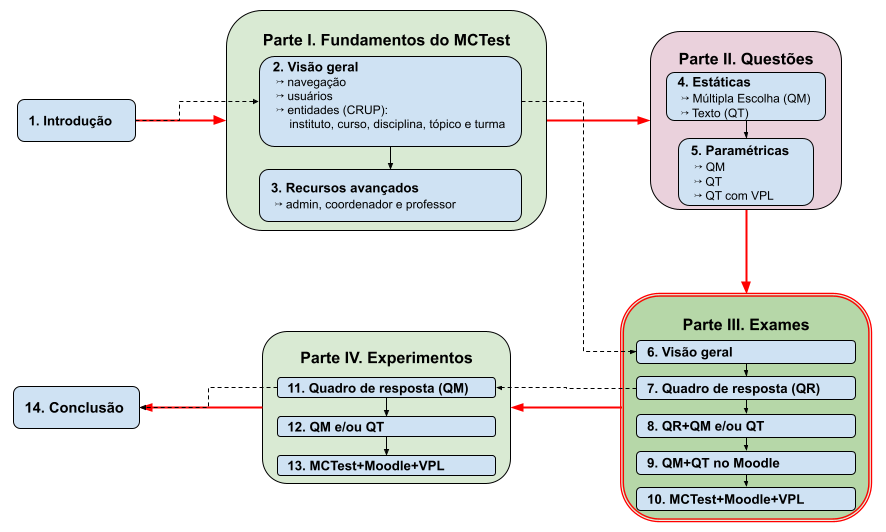
\includegraphics[width=1.00\textwidth]{cap01_MCTest-book-v3.png}\vspace{-0mm}
  \caption{Organização do livro.}
  \label{fig:cap01_MCTest-book}
\end{figure}

\begin{description}
    
\item[Parte \ref{part:fundamentos} -- Fundamentos do MCTest:] apresenta a introdução ao MCTest, seus componentes bási\-cos e funcionalidades essenciais. Esta parte inclui o Capítulo \ref{ch:visaoGeral} -- \nameref{ch:visaoGeral} e o Capítulo \ref{ch:metodosBasicos} -- \nameref{ch:metodosBasicos}, que abordam a visão geral do sistema, navegação, usuários e os métodos básicos de operação (CRUD -- \textit{Create, Read, Update, Delete}). As seções são dedicadas à manutenção de diferentes áreas do sistema por usuários administradores, coordenadores e professores.

\item[Parte \ref{part:questoesMCTest} -- Questões no MCTest:] trata de diferentes tipos de questões disponíveis no MCTest, como questões estáticas e paramétricas. Os Capítulos \ref{ch:questoesClassicasMCTest}  -- \nameref{ch:questoesClassicasMCTest} e \ref{ch:questoesCodigoMCTest} -- \nameref{ch:questoesCodigoMCTest} discutem questões de múltipla escolha (QMs), questões dissertativas ou de texto (QTs) e QTs com código.

\item[Parte \ref{part:exames} -- Exames no MCTest:] aborda o processo de criação e gerenciamento de exames no MCTest, com uma visão geral no Capítulo \ref{ch:exames} -- \nameref{ch:exames}. Os Capítulos \ref{ch:examesQR}  -- \nameref{ch:examesQR}, \ref{ch:examesQM_QT} -- \nameref{ch:examesQM_QT}, \ref{ch:examesQM_QT_Moodle} -- \nameref{ch:examesQM_QT_Moodle} e \ref{ch:examesQT_VPL} -- \nameref{ch:examesQT_VPL} exploram o quadro de respostas (QR) e a integração com questões de múltipla escolha (QMs) e/ou questões dissertativas (QTs), além da combinação do MCTest com Moodle e VPL para exames.

\item[Parte \ref{part:experimentos} -- Experimentos de Uso do MCTest:] apresenta \ estudos de caso \ e \ exemplos \ práticos do uso do MCTest em ambientes educacionais. Os Capítulos \ref{ch:experimentos_QR} -- \nameref{ch:experimentos_QR}, \ref{ch:experimentos_QR_QT} -- \nameref{ch:experimentos_QR_QT} e \ref{ch:experimentos_VPL} -- \nameref{ch:experimentos_VPL} apresentam diferentes cenários envolvendo o quadro de respostas (QR), questões de múltipla escolha (QMs) e/ou questões dissertativas (QTs) e a integração do MCTest com Moodle e VPL.

% \item[Parte \ref{part:questoesMoodle} -- Questões no Moodle:] foca na integração entre o MCTest e o Moodle, uma plataforma popular de aprendizado a distância. Os Capítulos \ref{ch:questoesClassicasMoodle} -- \nameref{ch:questoesClassicasMoodle}, \ref{ch:questoesCodigoMoodle} -- \nameref{ch:questoesCodigoMoodle} e \ref{ch:questoesMCTestMoodleVPL} -- \nameref{ch:questoesMCTestMoodleVPL} exploram diferentes tipos de questões, como questões clássicas, questões de código (VPL) e a combinação de MCTest, Moodle e VPL.  O leitor pode também pular essa parte se não desejar utilizar o Moodle.

% \item[Parte \ref{part:topicosAvancados} -- Tópicos Avançados:] aprofunda-se em aspectos técnicos do MCTest, como bibliotecas e instalações, arquitetura de software, banco de dados, visão computacional e segurança. Os Capítulos \ref{ch:bibliotecas} -- \nameref{ch:bibliotecas}, \ref{ch:arquitetura} -- \nameref{ch:arquitetura}, \ref{ch:bd}, \ref{ch:vc} -- \nameref{ch:vc} e \ref{ch:seguranca} -- \nameref{ch:seguranca} oferecem informações detalhadas sobre esses tópicos. O leitor pode pular essa parte se tiver como objetivo apenas utilizar o MCTest já implantado em sua instituição.

\end{description}

O livro é finalizado com o Capítulo \ref{ch:conclusao} -- \nameref{ch:conclusao}, que resume as principais ideias apresentadas ao longo do texto e oferece orientações para futuras pesquisas e desenvolvimentos do MCTest pela comunidade, visto que se trata de um sistema de código aberto. Esse capítulo é especialmente valioso para aqueles que desejam se aprofundar no tema e contribuir para o desenvolvimento contínuo do MCTest, seja por meio de pesquisas adicionais ou pela implementação de novas funcionalidades. Leitores interessados em utilizar o sistema exclusivamente para a elaboração e avaliação de exames que contenham apenas os QRs (as QMs serão apresentadas separadamente) devem seguir os capítulos indicados pelas setas tracejadas na Figura \ref{fig:cap01_MCTest-book}.